
%
%  $Description: Author guidelines and sample document in LaTeX 2.09$
%
%  $Author: ienne $
%  $Date: 1995/09/15 15:20:59 $
%  $Revision: 1.4 $
%

\documentclass[times, 10pt,twocolumn]{article}
\usepackage{latex8}
\usepackage{subfigure}
\usepackage{times}
\usepackage{amsmath,epsfig,longtable}
\usepackage[bf,belowskip=-15pt,aboveskip=-15pt,font=sf]{caption}
\renewcommand{\captionfont}{\normalsize}
%\renewcommand{\captionlabelfont}{\phv}
\setlength{\captionmargin}{0.17in}

%\documentstyle[times,art10,twocolumn,latex8]{article}

%-------------------------------------------------------------------------
% take the % away on next line to produce the final camera-ready version
\pagestyle{empty}

%-------------------------------------------------------------------------
\begin{document}

\title{Combining Evidence in Random Field Models Towards Validating Face Detection Results}

\author{Sreekar Krishna\thanks{Sreekar.Krishna@asu.edu; Ph: (480)326-6334; Fax: (480)965-1885}, and Sethuraman Panchanathan\\
School of Computing and Informatics (SCI) \\ Ira A Fulton School of
Computing \\ Arizona State University \\ Tempe, AZ - 85281 }

\maketitle
\thispagestyle{empty}

\begin{abstract}

\end{abstract}

%-------------------------------------------------------------------------
\Section{Introduction}\label{Introduction} Face detection has become
an important first step towards solving a plethora of other computer
vision problems such as face recognition, face tracking, pose
estimation, intent monitoring and other face related processing
[REF]. Over the years researchers have developed algorithms aimed at detecting faces in
front of complex backgrounds. Currently, the most popular face detection
algorithm is the Viola-Jones [REF] face detection algorithm,
whose popularity has been boosted by its availability in the form of
a speed-optimized C++ library
through the open source computer vision library, OpenCV [REF]).
Other face detection algorithms include [REF: GET A LIST HERE].


Most face detection algorithms learn faces by modeling the
intensity distributions in upright face images. These algorithms
tend to respond to face-like intensity
distributions in image regions that do not depict faces.
These spurious responses make the results unsuitable for further processing
that requires accurate face images as inputs, such as the ones
mentioned above. Figure \ref{Fig:ExampleFalseDetect} shows an
example where a face detection algorithm detects two faces - one
true and the other false.
\begin{figure}[h]
\centering
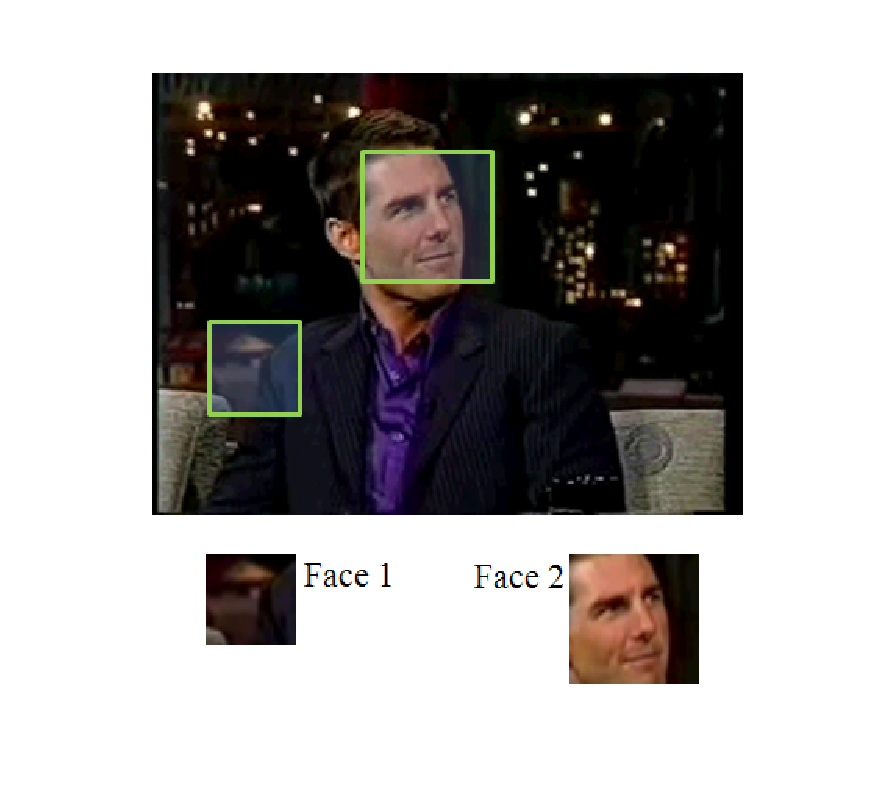
\includegraphics[width=3in]{Figure1.eps}
\caption{{\bf {\fontfamily{phv}\selectfont An example false face
detection using Viola-Jones [REF] face detection algorithm.}}}
\label{Fig:ExampleFalseDetect}
\end{figure}

The problem of false face detection has motivated some researchers
to develop heuristic approaches aimed for
validating the face detection results.
Section \ref{RelatedWork} details some of the more popular
heuristics for false face detection. Most of these heuristics
search for skin tones within the face detection output subimages.
However, this simple approach often fails to distinguish faces from non-faces,
because face detectors often fail to
center the cropping box precisely around the detected face. This produces a
significant patch of skin colored pixels, but only a partial face.
This centering problem can be dealt with by extracting the skin colored regions
and comparing their shape to an ellipse. While such heuristics,
are simple, and somewhat effective, their validation is not reliable
enough to meet the needs of higher level face processing tasks.
Further, they do not provide a confidence metric for their
validation.
\begin{figure}[h]
\centering
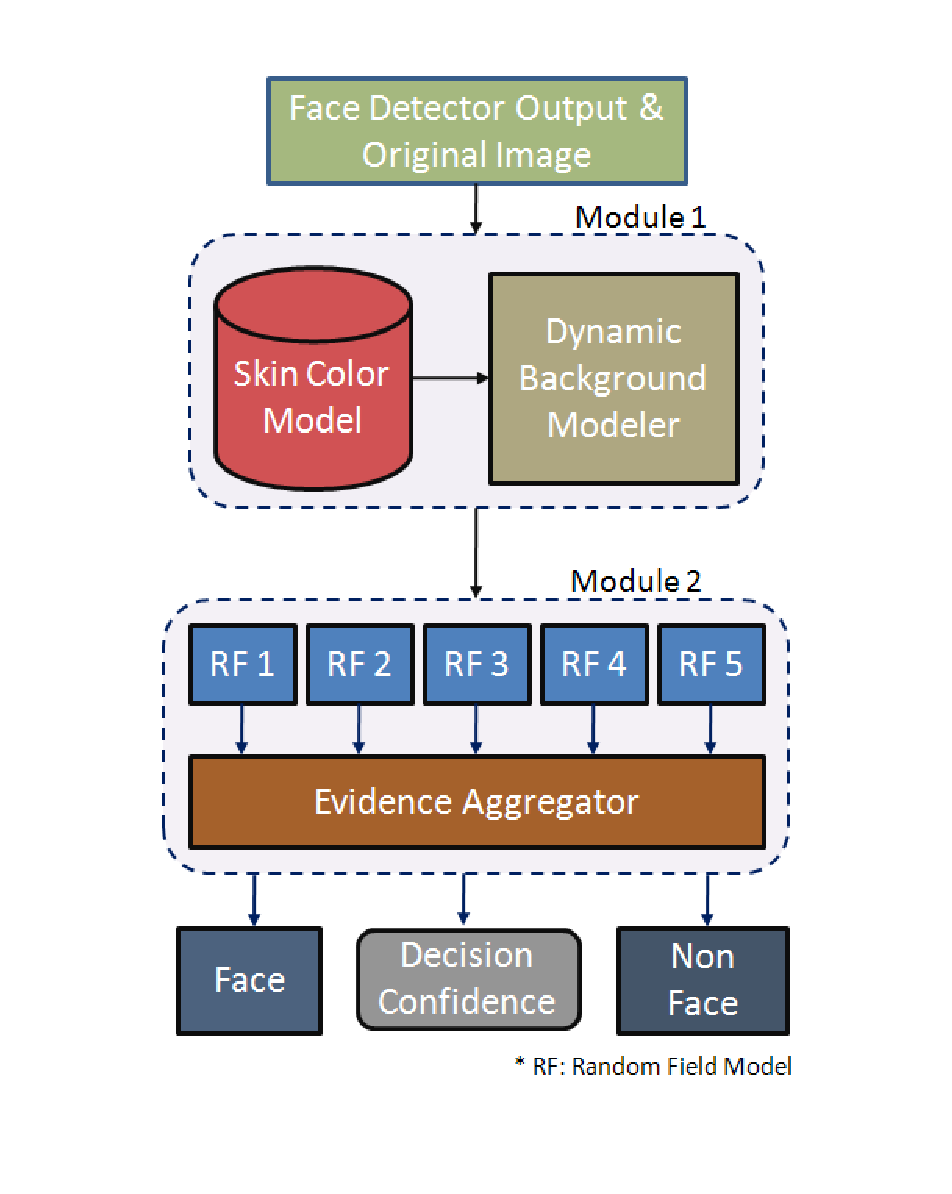
\includegraphics[width=3.5in]{Figure2.eps}
\caption{{\bf {\fontfamily{phv}\selectfont Block diagram of the
proposed framework for face detection validation.}}}
\label{Fig:BlockDiagram}
\end{figure}

This paper treats the problem of face detection validation in a
systematic manner, and proposes a learning framework that
incorporates both contextual and structural knowledge of human
faces. A face validation filter is designed by combining two
statistical modelers, 1) a human skin tone detector with a dynamic
background modeler (Module $1$), and 2) an evidence-aggregating
human face silhouette random field modeler (Module $2$), which
provides a confidence metric representing its validation of the
face. The block diagram in Figure \ref{Fig:BlockDiagram} shows the
functional flow of data through the two modules in the proposed
framework. The details of the statistical models and their learning
will be presented later in the paper, which is organized as follows.
Section 2 reviews some of the earlier research aimed at validating
face detection results. Section 3 introduces the proposed framework,
with details on the learning process. Section 4 discusses the data
used for training and testing the framework. Section 5 presents and
discusses the results, and Section 6 presents conclusions and a
discussion of future work.

%-------------------------------------------------------------------------
\Section{Related Work}\label{RelatedWork}

DO THIS SECTION SOON.

%-------------------------------------------------------------------------
\Section{Proposed Framework}\label{ProposedFramework} As Shown in
Figure \ref{Fig:BlockDiagram}, the framework essentially has two
statistically learnt models, Module $1$ and Module $2$, that are
cascaded to form the face detection validation filter. The output
from a face detector is sent to Module $1$, which
distinguishes the skin pixels in the face region from the
background pixels, thereby constucting a skin region mask.
This skin region mask then becomes the input to Module $2$, which is
essentially an aggregate of random field models learnt from manually
labeled ({\it true}) face detection outputs. The results of each
random field model within the aggregate are then combined, using
rules of Dempster-Shafer Theory of Evidence [REF]. This "combining of
evidence" provides a metric for the belief (i.e. confidence) of the system in its final
validation. The two modules are detailed in the
following subsections.
%-------------------------------------------------------------------------
\SubSection{Module $1$: Human Skin Tone Detector with Dynamic
Background Modeler}\label{Module1}

Most of the skin tone detectors [REF] used for human skin color
classification use prior knowledge, which is provided in the form of a
parametric or non-parametric model of skin samples that are
extracted from images - either manually, or through a semiautomated process. In this paper
we employ such an a priori model, in combination with a dynamic
background modeler, so that the skin vs. non-skin boundary is
accurately determined. Accurate skin region extraction is essential
for Module $2$, as it validates images based on their
structural properties. The two functional components of Module $1$
are:

\subsubsection{{\em a-priori} Bi-modal Gaussian Mixture Model
for Human Skin Classification}\label{Bi-ModGaussian} A normalized RGB
color space has been a popular choice among researchers for
parametric modeling of human skin color [REF]. The normalized RGB
(typically represented as nRGB) of a pixel $X$ with $X_r$, $X_g$,
$X_b$ as its red, green and blue components respectively, is defined
as:
\begin{equation}
X_{i|i \in \{r,g,b\}}^{(nRGB)} =
\frac{X_i}{\left(\sum\limits_{\forall_{i|i\in\{r,g,b\}}}X_i\right)}
\end{equation}
Normalized RGB space has the advantage that only two of the three
components, nR, nG or nB, is required at any one time to describe
the color. The third component can be derived from the other two as:
\begin{equation}
X_{i|i \in \{nR,nG,nB\}}^{(nRGB)} =  1 -\left(
\sum_{\forall_{k|(k\in\{nR,nG,nB\}, k \ne i)}}X_k \right)
\end{equation}
\vspace{-0.15in}
\begin{figure}[h]
\centering
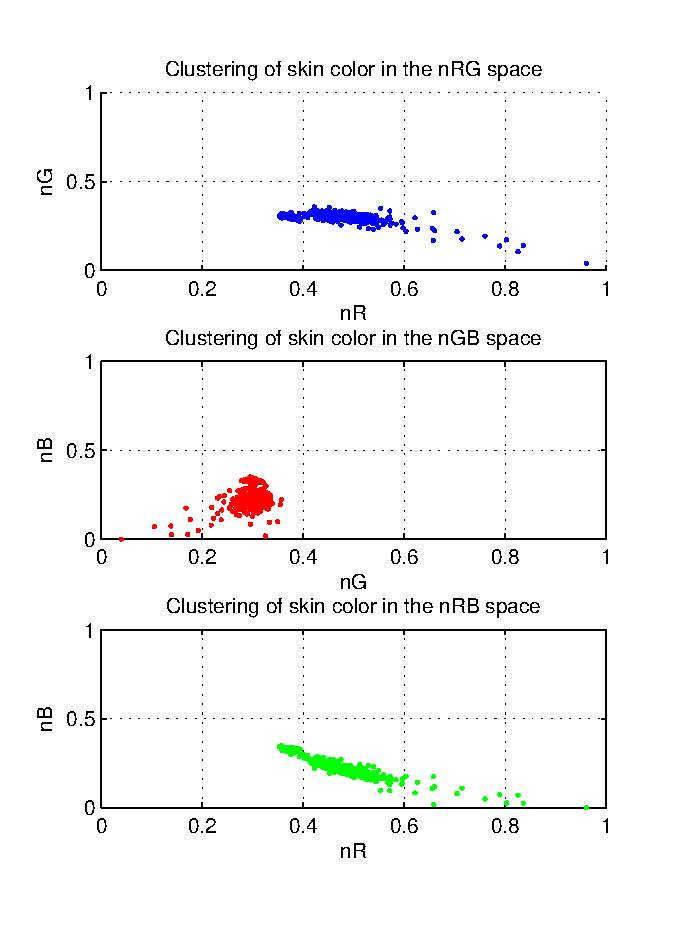
\includegraphics[width=3in]{Figure3.eps}
\caption{{\bf {\fontfamily{phv}\selectfont Projection of 1000
randomly sampled skin samples in three different nRGB spaces.\\}}}
\label{Fig:nRGBProject}
\end{figure}

In our experiments, we found that skin pixels form a tight cluster
when projected on nG and nB space, as shown in the Figure
\ref{Fig:nRGBProject}. The study was based on a skin pixel database,
consisting of nearly $150,000$ samples, built by randomly sampling
skin regions from $1040$ face images collected on the web as well as
from face databases such as FERET [REF]. Further analysis also showed
that the distribution of the samples in the 2D nG-nB space had two prominent density peaks
which motivated the modeling of skin pixels with a Bi-modal Gaussian
mixture model, which was learnt using Expectation Maximization (EM)[REF] with a
$k$-means initialization [REF] algorithm. The final modal is shown
in Figure \ref{Fig:BimodGaussian}. For the sake of completeness, we
provide the parameters of this Bi-modal Gaussian mixture, which was used in
our experiments.
\begin{eqnarray}
f^{skin}_{X|X=[nG,nB]}(x) & = & w_1 f_{Y_1}(x;\Theta_1=[\mu_1,\Sigma_1]) +  \nonumber  \\
       &  & w_2 f_{Y_2}(x;\Theta_2=\{\mu_2,\Sigma_2\})
\end{eqnarray}
where, $w_1 = 0.76$, $w_2 = 0.24$, $\mu_1 = [0.30,0.22]$, $\mu_2 =
[0.3, 0.32]$, $\Sigma_1=\left[ \begin{array}{cc} 0.024 & 0
\\ 0.017 & 0.03\end{array}\right]$, $\Sigma_2=\left[ \begin{array}{cc} 0.007 & 0
\\ -0.0016 & 0.0058\end{array}\right]$
\vspace{-0.15in}
\begin{figure}[h]
\centering
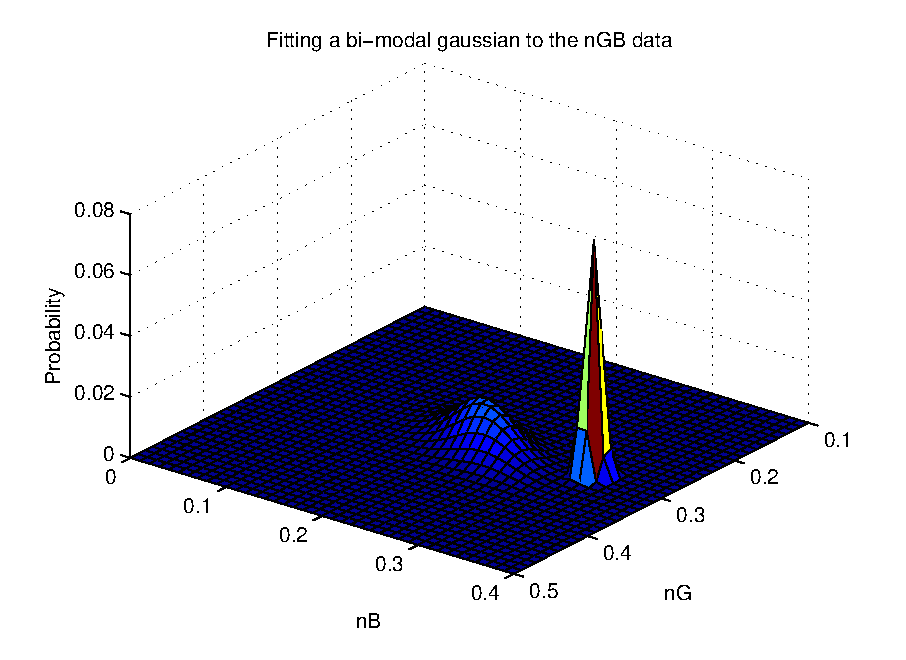
\includegraphics[width=3.5in]{Figure4.eps}
\caption{{\bf {\fontfamily{phv}\selectfont \\ Bi-modal Gaussian
fitting to skin color pixels on a nG-nB space}}}
\label{Fig:BimodGaussian}
\end{figure}
\subsubsection{Dynamically Learnt Multi-modal Gaussian Model for
Background Pixel Classification}\label{DynamicModel} As mentioned
earlier, classification of regions into face or
non-face regions requires accurate skin vs. non-skin classification. In
order to achieve this, we learn the background color surrounding each face
detector output dynamically. To this end we extract an extra region
of the original image around the face detector's output, as shown in
Figure \ref{Fig:Extraregion}. Since the size of the face detector output
varies from image to image, it is necessary to normalize the size.
This is done by downsampling the size of the original image, to produce
a face detector output region containing 90x90 pixels.  The extra region
pixels surrounding the face are then extracted from the 100x100 region
around this 90x90 normalized face region.
\vspace{-0.15in}
\begin{figure}[h]
\centering
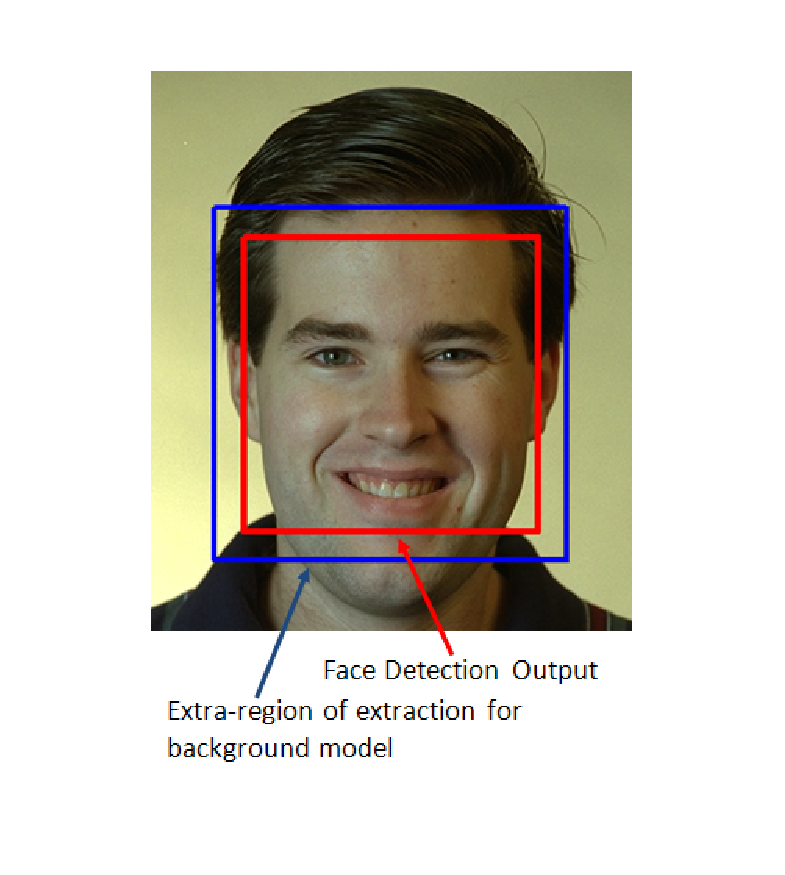
\includegraphics[width=2.5in]{Figure5.eps}
\caption{{\bf {\fontfamily{phv}\selectfont Extraction of extra
region around the face detector output to learn the background
model.}}} \label{Fig:Extraregion}
\end{figure}

Once the outer pixels are extracted, a Multi-modal Gaussian Mixture model
is trained using EM with $k$-means initialization, similar to the
earlier case with the skin pixel model. The resulting model can be
represented as:
\begin{equation}
f^{non-skin}_{X|X=[R,G,B]}(x) =
\sum\limits_{i=1}^{m}w(i)f_{Y_i}\left(x;\Theta_i=[\mu_i,\Sigma_i]\right)
\end{equation}
where, $m$ is the number of Gaussians in the mixture model.
Because the backgrounds in the images that we used were fairly simple,
we found empirically that a value of $m=2$ or $m=3$
modeled the backgrounds with sufficient accuracy.

\subsubsection{Skin and Background Classification using the learnt
Multi-modal Gaussian Models}\label{SkinnBackground} The skin and
non-skin models, $f^{skin}_{X|X=[nG,nB]}(x)$ and
$f^{non-skin}_{X|X=[R,G,B]}(x)$ respectively, are used for
classifying every pixel in the scaled face image obtained as
explained in the Section \ref{DynamicModel}. An example skin-mask
is shown in Figure \ref{Fig:Skinmasks}. This example shows two sets
of images - one corresponding to a {\it true} face detection result, and
another {\it false} face detection result. \vspace{-0.15in}
\begin{figure}[h]
\hspace{-0.4in}
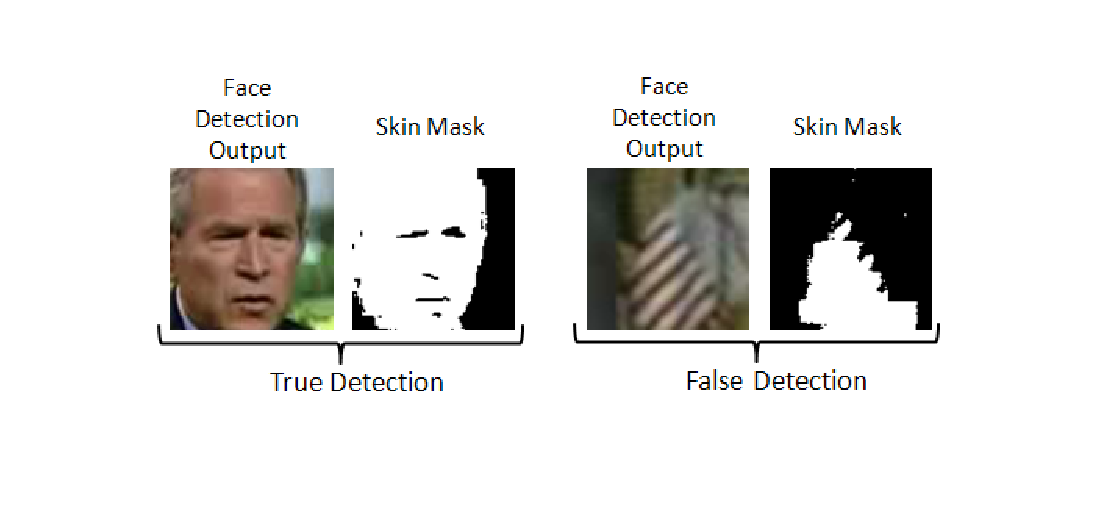
\includegraphics[width=4in]{Figure6.eps}
\caption{{\bf {\fontfamily{phv}\selectfont Example of {\em true} and
{\em false} face detection results, with their corresponding skin
masks extracted as described in Section \ref{DynamicModel}}}}
\label{Fig:Skinmasks}
\end{figure}


%-------------------------------------------------------------------------
\SubSection{Module $2$: Evidence-Aggregating Human Face Silhouette
Random Field Modeler}\label{Module2} The structural analysis
through Random Field models detailed in this section
will describe how the evidence agrregator
is used to distinguish between the {\it true} and {\it false} face detections shown
in Figure \ref{Fig:ExampleFalseDetect}. In order to validate the skin
region extracted as explained in Section \ref{Module1}, we build
statistical models from examples of faces. To this end we
chose Markov Random Fields (MRF) to capture the variations possible
in {\it true} skin masks (face silhouette). The following
subsections details the process.

\subsection{Markov Random Fields}\label{MRF}
MRFs encompass a class of probabilistic image analysis techniques
that rely on modeling the intensity variations and interactions
among the image pixels. MRFs have been widely used in low level
image processing including, image reconstruction, texture
classification and image segmentation [REF from texture
classification paper]. In this work, we use MRFs to learn the
structure of a {\it true} face skin mask.

In an MRF, the sites in a set, $\mathcal S$, are related to one
another via a neighborhood system, where a neigborhood is defined as ${\mathcal
N}=\{{\mathcal N}_i, i \in \mathcal S\}$, where ${\mathcal N}_i$ is
the set of sites neighboring $i$, $i \notin {\mathcal N}_i$ and $i
\in {\mathcal N}_j \Longleftrightarrow j \in {\mathcal N}_i$.

A random field X said to be an MRF on $\mathcal S$ with respect to a
neighborhood system $\mathcal N$, if and only if,
\begin{eqnarray}&& P({\mathbf x})>0, \forall \mathbf x \in \mathcal X  \\ && P(x_i\vert x_{{\mathcal S}-\{i\}})=P(x_i\vert x_{{\mathcal N}_i}) \label{Eqn:5} \end{eqnarray}
where, $P(x_i\vert x_{{\mathcal S}-\{i\}}$ represents a Local
Conditional Probability Density function defined over the
neighborhood $\mathcal N$.

In our experiments we found out that modeling the skin-region
validation problem into one single MRF gave poor results. We devised
$5$ unique Random Field models with an Dempster-Shafer Evidence
aggregating framework that could not only validate the face
detection outputs, but also provide a metric on its confidence in
the validation. Thus, Equation \ref{Eqn:5} could be alternatively
seen as a set $P({\mathbf x}) = \{P^1({\mathbf x}), \ldots,
P^5({\mathbf x})\}$, each having their own neighborhood system
$\mathcal N^k = \{\mathcal N^1, \mathcal N^2, \ldots, \mathcal
N^5\}$, such that
\begin{equation}
P^k(x_i\vert x_{{\mathcal S}-\{i\}})=P(x_i\vert x_{{\mathcal
N^k_i}})
\end{equation}

\subsubsection{Pre-processing}\label{Preprocessing}As described earlier,
each face detector output is normalized and expanded to produce a $100$x$100$ pixel image,
from which a $100$x$100$ binary skin mask is generated.
A morphological opening and closing operation is then performed on the skin mask, and the
mask is then partitioned into 100 $10$x$10$ blocks, as shown in Figure
\ref{Fig:RowColumnBlocks}.  Each block contains 100 binary pixels.  The number of white mask
pixels
(which represent skin pixels) are counted in each block, and a $10$x$10$ matrix is constructed,
where
each element of this matrix contains a number between 0 and 100.
This $10$x$10$ matrix is then used as the basis for determining whether the face detector output
is indeed a face.

\begin{figure}[h]
\hspace{-0.3in}
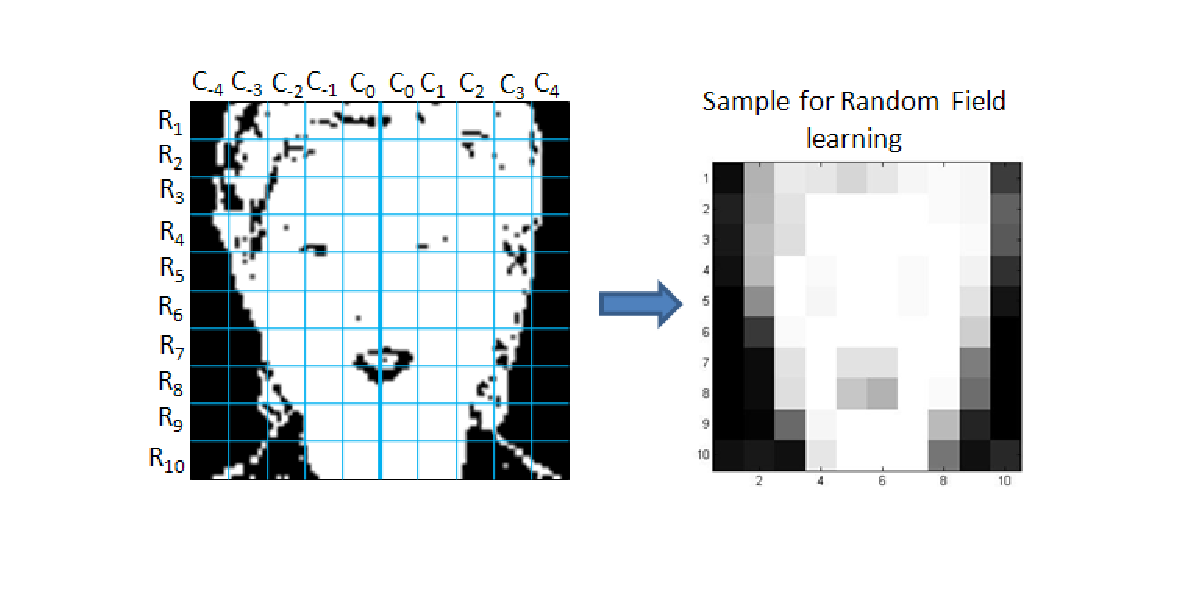
\includegraphics[width=4in]{Figure7.eps} \caption{{\bf
{\fontfamily{phv}\selectfont }}} \label{Fig:RowColumnBlocks}
\end{figure}

\subsubsection{Symmetry estimation}\label{Symmetry}The determination of whether the
face detector output is actually a face is based on heuristics that are derived from anthropological human face
models [REF] and through our own statistical analysis. These include:
\begin{enumerate}
\item Human faces are horizontally symmetrical (i.e. along any row of blocks $R_i$)
about a  central vertical line joining the nose bridge, the tip of the nose and the chin cleft, as
shown in Figure \ref{Fig:RowColumnBlocks}.  In particular, our analysis of a large set
of frontal face images showed that the counts of skin pixels
in the 10 blocks that form
each row in Figure \ref{Fig:RowColumnBlocks}
were roughly symmetrical across this central line.
\item Variations in the numbers of skin pixels per block along the verticals ($C_i$'s) are substantial enough that
each row of blocks $R_i$ contributes some additional independent evidence about the symmetry of the face image.
The symmetry of the image was estimated by computing the differences between
the pixel counts

\ref{Fig:Neighborhood}.
\end{enumerate}

\begin{figure}[h]
\hspace{-0.3in}
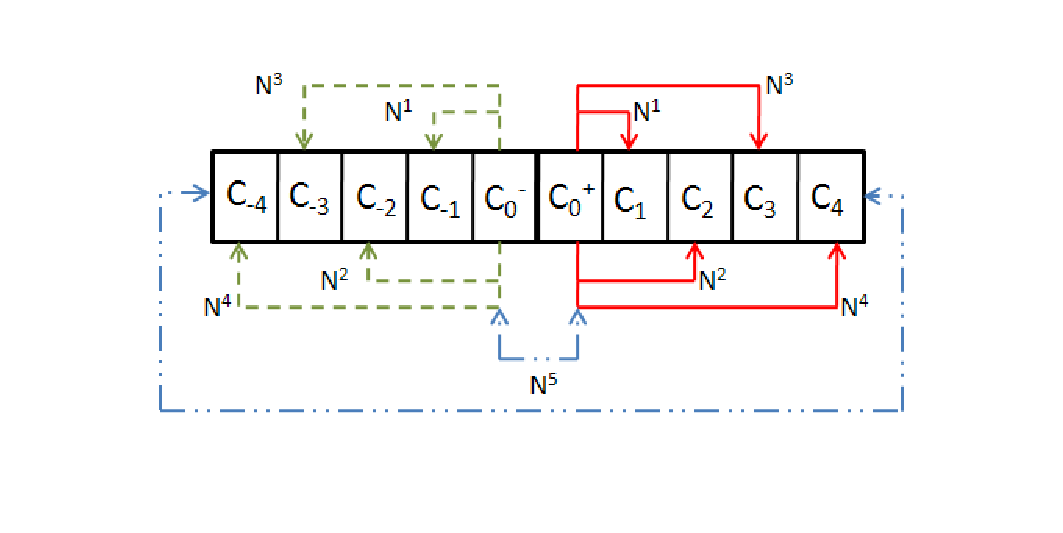
\includegraphics[width=4in]{Figure8.eps} \caption{{\bf
{\fontfamily{phv}\selectfont }}} \label{Fig:Neighborhood}
\end{figure}

The different neighborhood systems $\mathcal N^k$ can be defined as
(Refer Figure \ref{Fig:Neighborhood}):
\begin{equation}
\mathcal N^k = \left\{C_{j | j \in \{|k|, 0^-, 0^+\}}\right\}
\end{equation}

\subsubsection{Local Conditional Probability Density (LCPD)}\label{LCPD} To model the
variations on the skin-region mask, we choose to build 2D histogram
over the various neighborhood systems such that the two dimensions
capture the various structural properties of {\it true} skin masks.
The two dimensions will become apparent once the definitions are
introduces below. Further, since we chose to model the variations
into $5$ different MRFs, this requires $5$ different histogram
definitions.
\begin{itemize}
\item $\mathbf{H}^{k|k=\{1,2,3,4\}} = \left\{ \mathbf{z}\right\}$, where,
\begin{equation}\mathbf{z} = [x_{C_{0^{\pm}}}, \delta(x_{C_{0^{\pm}}},
x_{C_{\pm k}})] , \forall R_{j} \label{Eqn:9}
\end{equation}

\item$\mathbf{H}^{k=5} = \left\{
\mathbf{z}\right\}$, where,
\begin{equation}
\mathbf{z} = [\mu(x_{C_{0^+}},x_{C_{0^-}}), \mu(x_{C_{-4}},
x_{C_{+4}})] , \forall R_{j} \label{Eqn:10}
\end{equation}
\end{itemize}

where, $\mathbf{H}^k$ is the 2D histogram pool, $x_{C_k}$ is the
value on the skin mask at location $C_k$. The two functions
$\delta(.,.)$ and $\mu(.,.)$ can be represented as
\begin{eqnarray}
\delta(x_{C_{0^{\pm}}}, x_{C_{\pm i}}) & = & \left\{
\begin{array}{l l}
x_{C_{0^+}} - x_{C_{+i}}, & i>0 \\
x_{C_{-i}} - x_{C_{0^-}}, & i<0 \\
\end{array}
\right. \\
\mu(a,b) & = & \frac{a+b}{2}
\end{eqnarray}
In order to estimate the LCPD on these $5$ histogram pools, we use
Parzen Window Density Estimation (PWDE) technique [REF] with a 2D
Gaussian window. Thus, each of LCPD can now be defined as
\begin{equation}
P^k(\mathbf z) = \frac{1}{(2\pi)^{d/2} n
h_{opt}^d}\sum\limits_{j=1}^n \exp \left[-\frac{1}{2 h^2_{opt}}
\left(\mathbf{z} - \mathbf {H}^k_j\right)^T \Sigma^{-1} \left(
\mathbf{z} - \mathbf {H}^k_j\right) \right]
\end{equation}
where, $n$ is the number of samples in the histogram pool
$\mathbf{H}^k$, $d$ is number of dimensions (in our case $2$),
$\Sigma$ and $h_{opt}$ are the covariance matrix over $\mathbf{H}^k$
and the optimal window width respectively. They are defined as:
\begin{eqnarray}
\Sigma = \left[\begin{array}{cc} \sigma_{dim1} & 0 \\ 0 &
\sigma_{dim2}\end{array} \right], & h_{opt} =
\frac{\sigma_{dim1}+\sigma_{dim2}}{2} \left\{\frac{4}{n(2d+1)}
\right\}^{1/(d+4)}          \nonumber
\end{eqnarray}
Figure \ref{Fig:LCPDs} shows the $5$ LCPDs learnt over a set of
$390$ training face images.
\begin{figure}[h]
\hspace{-0.3in}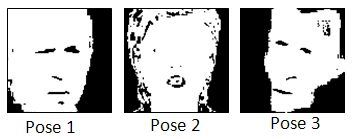
\includegraphics[width=4in]{Figure9.eps}
\caption{{\bf {\fontfamily{phv}\selectfont }}} \label{Fig:LCPDs}
\end{figure}
\subsubsection{Human Face Pose}\label{HumanFacePose}During our studies we discovered that
the cropping on the face changes based on the pose of the head. This
is evident in Figure \ref{Fig:PoseMasks}. Combining face examples
from these sets into one set of MRFs seem to dilute the LCPDs and
the discriminating capabilities reseeded. This motivated us to
design three different sets of MRFs, one for each of pose form as
shown in the figure. These pose forms could broadly classified as 1.
Turned right ($r$), 2. Facing front ($f$), and 3. Turned Left ($l$).
\begin{figure}[h]
\hspace{-0.3in}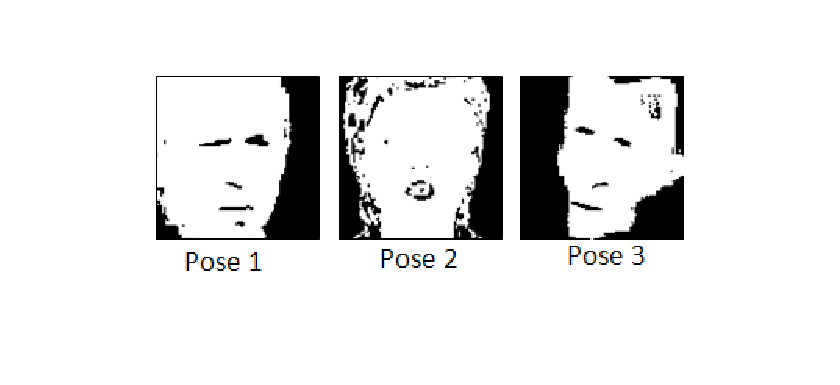
\includegraphics[width=4in]{Figure10.eps}
\caption{{\bf {\fontfamily{phv}\selectfont }}} \label{Fig:PoseMasks}
\end{figure}
Thus, the final set of LCPDs could be described by the super set.
\begin{equation}
P(\mathbf z) = \left\{P^{k|k=\{1,\ldots,5\}}_{m|m=\{r,f,l\}}(\mathbf
z) \right\}
\end{equation}
\subsection{Summary}\label{Summary}
Given any test face detection output, the consecutive steps towards
a decision could be summarized in a list as:
\begin{enumerate}
\item Input face detection output into Module 1 for a skin-region
mask as described in Section \ref{Module1}.
\item Apply morphological operators to the skin mask and obtain a sub-sampled
$10$x$10$ image as described in Section \ref{Module2}.
\item Extract $\mathbf{z}$ as described in Equation \ref{Eqn:9} and \ref{Eqn:10}.
\item Project $\mathbf{z}$ on the LCPD set $P(\mathbf z)$ to get a
set of likelihoods $l_m^k$.
\end{enumerate}
In order to make decision on the face detection result, it is
essential that the various likelihoods be combined into a certain
result. Towards this end we use the Dempster-Shafer theory of
evidence as explained in the next subsection. Before combining the
results, the likelihoods obtained as explained in Section
\ref{Summary} are converted into their log-likelihood equivalents as
$L_m^k = \ln \left(l_m^k\right)$.
\subsection{Combining Evidence}\label{CombiningEvidence}
Given any test face detection result, a clear decision on acceptance
or rejection of the image as being face or not can be done only by
setting a threshold on the Log-likelihood value that the test face
generates on the LCPD set $P(\mathbf z)$. Given there are five LCPD
per face pose and $3$ sets of face poses, we incorporated (through
observation) a piece-wise linear decision model instead of a hard
threshold on the acceptance of a face image as true or not. This is
illustrated in the Figure \ref{Fig:Thresholds}. Each LCPD
$P^k(\mathbf z)$ was provided with an upper and lower threshold of
acceptance and rejection respectively. The upper and lower bounds
were obtained by observing $P^k(\mathbf z)$ for the three face poses
$P^k_{r,f,l}(\mathbf z)$. Thus, any log-likelihood values lesser
than the lower threshold ($L_L$) would result in $P^k(\mathbf z)$
deciding against the test input, while any log-likelihoods greater
that the upper threshold ($L_U$) would be a certain accept. Anything
in between would be assigned a probability of acceptance.
\begin{figure}[h]
\centering
\hspace{-0.3in}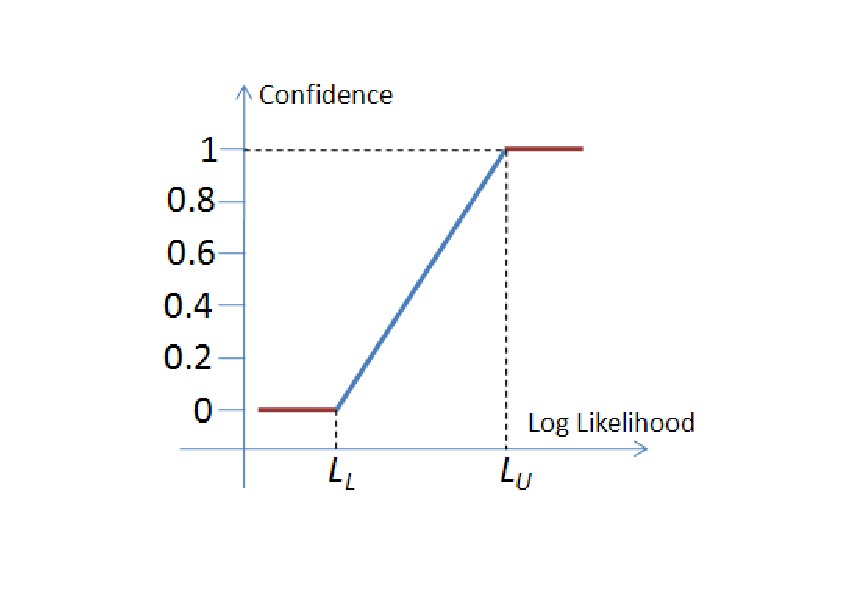
\includegraphics[width=2.5in]{Figure11.eps}
\caption{{\bf {\fontfamily{phv}\selectfont }}}
\label{Fig:Thresholds}
\end{figure}
In order to combine the net result of the five LCPD $P^k(\mathbf Z)$
decisions, we resort to Dempster-Shafer Theory of Evidence.
\subsubsection{Dempster-Shafer Theory of Evidence (DST)}\label{DST}
The Dempster-Shafer theory is a mathematical theory of evidence
[REF] which is a generalization of probability theory with
probabilities assigned to sets rather than single entities. Let $X$
be the universal set. The power set, $\mathbf{P}(X)$, is the set of
all possible sub-sets of $X$, including the empty set $\emptyset$.
The theory of evidence assigns a belief mass to each subset of the
power set through a  a function called the basic belief assignment
(BBA), $m:\mathbf{P}(X) \rightarrow [0,1]$, when it verifies two
axioms.
\begin{enumerate}
\item $m(\emptyset)$ = 0
\item $\sum\limits_{\mathbf{A} \in \mathbf{P}(X)} m(\mathbf{A})= 1$
\end{enumerate}
The mass $m(A)$ of a given member of the power set, expresses the
proportion of all relevant and available evidence that supports the
claim that the actual state belongs to $A$ but to no particular
subset of $A$. \\
{\em Rules of Combination}: The potential use of DST in our
application becomes clear with the rules of combining evidence which
was proposed as an immediate extension of DST. The combined mass
(evidence) of any two experts opinions, $m_1$ and $m_2$, can be
represented as:
\begin{eqnarray}
m_{1,2}(\emptyset) & = &  0 \\
m_{1,2}(A)& =  & \frac{1}{1-K}\sum\limits_{B\cap C = A, A \ne
\emptyset}m_1(B) m_2(C) \label{Eqn:16}
\end{eqnarray}
where,
\begin{equation}
K = \sum\limits_{B \cup C = \emptyset}m_1(B) m_2(C) \label{Eqn:17}
\end{equation}
$K$ is a measure of the amount of conflict between the two experts.
The normalization factor, $(1-K)$, has the effect of completely
ignoring conflict and attributing any mass associated with conflict
to a null set.

In our experiments, we treated the mapping shown in Figure
\ref{Fig:Thresholds} as the mass $m$ and each of the $5$ LCPDs,
$P^k(\mathbf z)$ were considered as experts towards voting on the
test input as a face or non-face. In order to use these mapped
values in Equation \ref{Eqn:16} - \ref{Eqn:17}, we normalized
evidences generated by the experts to map between $[0,1]$ and any
conflict of opinions were added into the factor $K$. For the sake of
clarity, we show an example of combining two expert opinions in
Figure \ref{Fig:DST}. The same idea could be extended to multiple
experts.
\begin{figure}[h]
\centering
\hspace{-0.2in}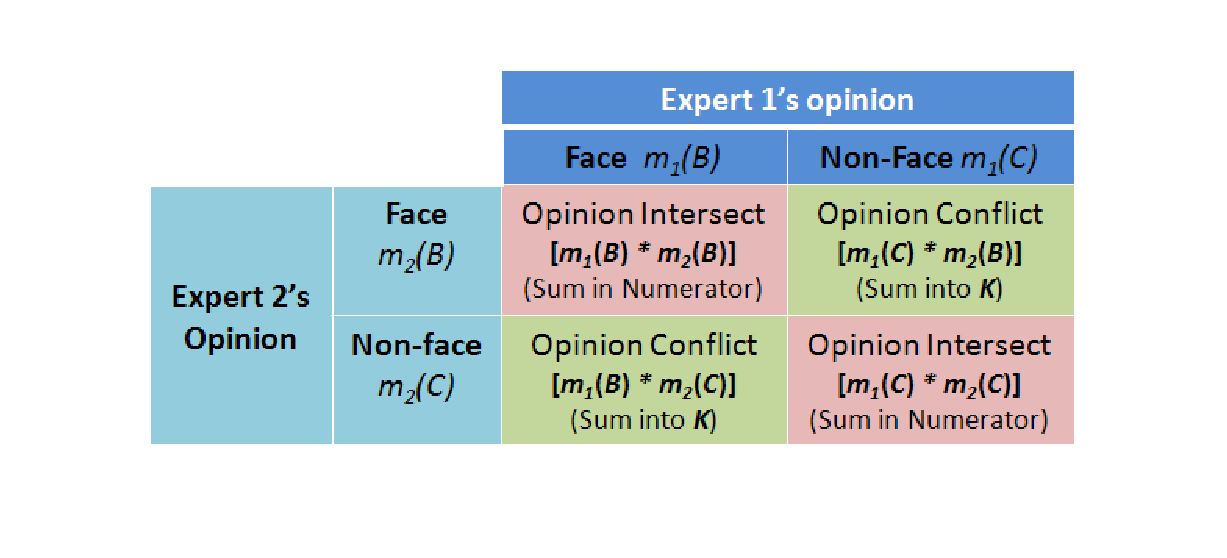
\includegraphics[width=3.5in]{Figure12.eps}
\caption{{\bf {\fontfamily{phv}\selectfont }}} \label{Fig:DST}
\end{figure}

\subsection{Coarse Pose estimation}\label{CoarsePoseEstimation}
Sice we used the various pose information to model the face
structure, we also investigated the possibility of determining the
pose of the face based on the evidences obtained with the LCPDs. We
noticed that the LCPDs $P^3(\mathbf z)$, $P^4(\mathbf z)$ and
$P^5(\mathbf z)$ were efficient in not only discriminating faces
from non-faces, but also the pose of the face into $3$ classes, 1.
Looking right, 2. Frontal and 3. Looking Left. Due to space
constraint, the procedure is not explained in detail, but it was
similar to what was followed for face versus non-face discrimination
as explained in Section \ref{CombiningEvidence}.

%-------------------------------------------------------------------------
\Section{Experiments}\label{Experiments} Two data sets of face
images were used in all our experiments.
\begin{enumerate}
\item The FERET Color Face Database
\item An in house face video database consisting of $17$ video
interviews collected over the web. The videos were of varying length
of time and accounted for nearly $2300$ frames containing face
images.
\end{enumerate}
As mentioned before, Viola-Jones face detection algorithm was used
in all our experiments. In order to prepare the data for processing,
face detection was performed on all the images in both the data
sets. The number of face detection do not directly correlate to the
number of unique face images as there are plenty of false
detections. We manually identified each and every face detection to
be {\it true} or {\it false} so that ground truth could be
established. The details of this manual labeling is shown below:
\begin{enumerate}
\item {\em FERET}
\begin{itemize}
\item Number of actual face images:
\item Number of faces detected using Viola-Jones algorithm:
\item Number of {\it true} detections:
\end{itemize}
\item {In house database}
\begin{itemize}
\item Number of actual face images:
\item Number of faces detected using Viola-Jones algorithm:
\item Number of {\it true} detections:
\end{itemize}
\end{enumerate}


%-------------------------------------------------------------------------
\Section{Results and Discussions}


%-------------------------------------------------------------------------
\Section{Conclusions and Future Work}


%-------------------------------------------------------------------------
\nocite{ex1,ex2}
\bibliographystyle{latex8}
\bibliography{latex8}

\end{document}
